\documentclass[fleqn]{article}

\usepackage{amsmath, amsthm, amssymb}
\usepackage{geometry}
\geometry{margin = 3.0 cm}

\usepackage{enumerate}
\usepackage{url}
\usepackage{listings}
\usepackage{color}

\usepackage{tikz}
\newcommand*\circled[1]{\tikz[baseline=(char.base)]{
            \node[shape=circle,draw,inner sep=2pt, color=red] (char) {#1};}}

\newcommand*\circledt[1]{\tikz[baseline=(char.base)]{
            \node[shape=circle,draw,inner sep=2pt, color=blue] (char) {#1};}}


\usepackage{algorithm}
\usepackage{caption}
\usepackage{algpseudocode}
\algblockdefx[NAME]{Input}{EndInput}
    [1][]{\textbf{Input:} #1}
    {}

\algblockdefx[NAME]{Output}{EndOutput}
    [1][]{\textbf{Output:} #1}
    {}

\newcommand{\myalg}[2]{\begin{figure}[H]
    { \renewcommand{\figurename}{Algorithm}
\begin{center}
\begin{minipage}{0.6\textwidth}
\hrulefill
\begin{algorithmic}[1]
    #1
\end{algorithmic}
\hrulefill
\end{minipage}
\end{center}
\caption{#2}
}
\end{figure}}

\renewcommand{\l}{\lambda}
\renewcommand{\L}{\Lambda}
\renewcommand{\mod}{~\mathrm{mod}~}
\renewcommand{\div}{~\mathrm{div}~}

\renewcommand{\vec}[1]{\mathbf{#1}}

\renewcommand{\(}{\left(}
\renewcommand{\)}{\right)}

\newcommand{\dist}{\text{dist}}
\newcommand{\todo}[1]{\textcolor{red}{#1}}

\newcommand{\mat}[1]{\begin{pmatrix} #1 \end{pmatrix}}
\newcommand{\room}{\hspace{0.5cm}}
\newcommand{\hl}[1]{\textbf{#1}}
\newcommand{\ceil}[1]{\lceil #1 \rceil}
\newcommand{\floor}[1]{\lfloor #1 \rfloor}

%\newcommand{\tm}{\textsuperscript{\texttrademark}}
\def\tm{$^{\hbox{\tiny TM}}$~}

\newtheorem{lem}{Lemma}

\usepackage{tikz} \usetikzlibrary{shapes}
\usetikzlibrary{arrows}

\tikzset{node distance=3cm, auto}

\lstset{language=C++,
                basicstyle=\ttfamily,
                keywordstyle=\color{blue}\ttfamily,
                stringstyle=\color{red}\ttfamily,
                commentstyle=\color{green}\ttfamily,
                morecomment=[l][\color{magenta}]{\#}
}

\title{\textsc{Implementation of the BSP model for the Epiphany\tm architecture}}
\author{Jan-Willem Buurlage \ Abe Wits \\ \normalsize{Utrecht University, The Netherlands}}

\begin{document}

\maketitle

\abstract{In this report we introduce the \texttt{epiphany-bsp} library, an implementation of the BSP model on the Epiphany\tm architecture. After introducing this architecture, we give some technical details of current hardware that ship with an Epiphany\tm chip. Next we describe the BSP library that we developed.}

\tableofcontents

\newpage

\setlength{\parskip}{0.2 cm}
\setlength{\parindent}{0.0 cm}
\setlength{\mathindent}{1.0 cm}

\section{Introduction}

The Epiphany\tm architecture is a multi-core microprocessor architecture that was developed by Adapteva\footnote{\url{http://www.adapteva.com}}. The Epiphany\tm architecture is implemented on chips that are inteded as a coprocessor to ARM/Intel CPUs. Every core has access to local, and shared memory. Besides the Epiphany\tm technology Adapteva has developed the Parallella board\footnote{\url{http://www.parallella.org}}, which is a computer with the size of a credit card that is based on this multi-core coprocessor technology.

\subsection{The Epiphany\tm architecture}

The Epiphany\tm architecture consists of 1 to 4096 Reduced Instruction Set Computer (RISC) cores, with local memory. These cores are part of a multi-core framework. Besides this there is a Network-On-Chip (NOC) present, designed for real time applications. \ldots

\subsubsection{Memory model}



\section{Parallella Board}

Toy model, new architecture

\subsection{Memory}

We will devide the Parallella board into a global and a local part:

\begin{tabular}{l|ll}
Scope & Global & Local \\
\hline
Processor & ARM & Epiphany\tm \\
Library & eHAL & eLib \\
Memory & 1 GB & 32 KB \\
Alloc & e\_alloc & ... \\
Get & e\_read & e\_read \\
Put & e\_write & e\_write \\

\end{tabular}

Note that only a very small amount of memory is available locally! This small local cache also contains the executable, leaving little memory for our algorithm; the Hello World implementation provided by Adapteva has a binary of 14KB, that is more than 40 percent of the memory available locally. The global memory can be used to store larger variables, but doing this in an efficient way is non-trivial and does not adhere to the BSP-model. One possible way to use bigger programs is to split it into several smaller programs, leaving supersteps intact. The cost of loading a new program image could be seen as additional synchronisation cost, increasing $l$.

Direct communication between cores is essential to the BSP model; if all communication has to go through the ARM processors and/or local memory, the central assumption that communication speed is determined by the largest amount of data sent/received by one processor breaks down. Instead we would get (semi)linear behaviour, reducing the advantages of parallel computing. Also, efficient usage of the Parallella board would require thoughtful modification of the regular optimal BSP-algorithms. 

\subsubsection{Variable registration}
First we will handle how variable registration works in BSP:
\\
\begin{lstlisting}
void bsp_push_reg (const void *ident, int size);
void bsp_put(int pid,const void *src,void *dst,int offset,int nbytes);
\end{lstlisting}
Above are the BSP commands to register a variable and to put some value in a registered variable.
All processors have to register a variable in the same superstep. BSP will ``tie together'' the pointers passed in \texttt{bsp\_push\_reg}; they are assumed to all point to a local version of the same variable. We will give this set of variables an index, \texttt{slotID}. Then if we use \texttt{bsp\_put}, we pass a local pointer \texttt{*dst} and a \texttt{\texttt{pid}}; they form an adress to the local version of \texttt{*dst} in processor \texttt{pid}. To be able to give this adress, we need some mapping of \texttt{*dst} to all the pointers with the same \texttt{slotID}; this implies they were registered in the same superstep. Then we need to take the pointer that is local to processor \texttt{pid}.
\\
If a normal (non-tiny) amount of memory is available, we could for example write the required data structures in C++ like this:
\begin{lstlisting}
map<void*, int> pointer_to_slotID;
vector<vector<int> > registered_variables;
\end{lstlisting}
Given \texttt{*dst} and \texttt{pid}, we can now give the actual pointer to the version of \texttt{*dst} local to processor \texttt{pid}:
\begin{lstlisting}
int slotID = pointer_to_slotID[dst];
void* actual_destination=registered_variables[slotID][pid];
\end{lstlisting}
With this approach, we need only $\mathcal{O}(\log(n))$ time to get the correct \texttt{slotID}, and we can then get \texttt{actual\_destination} in $\mathcal{O}(1)$ time. The std::map and std::vector datastructures are of variable size and allow fast insertion. However, they do have some memory-overhead; std::map is implemented as a red-black tree, and needs $48+(32+size)*length$ bytes (in GNU 64 bit C++ library), $size$ is of order 8 bytes (\texttt{sizeof(void*)+sizeof(int)}). When we register 10 variables, the map will use ~500 bytes. A vector uses approximately $24+size*length*2$ bytes, our vector of vectors will use order 4KB if we use 16 processors and we register 10 variables. To put this in perspective; on our Epiphany this map and vector use respectively 2 and 13 percent of the available memory!\\
\\
Instead we use only one datastructure:
\begin{lstlisting}
void*** registermap;
\end{lstlisting}
\texttt{registermap[slotID][pid]} is the pointer to the \texttt{slotID}th variable in processor pid.
We get the correct \texttt{slotID} by finding \texttt{*dst} among all variables registered by our current processor, this takes $\mathcal{O}(n)$ time, but since it is very likely that $n$ is small, this is acceptable. It is not as flexible; to resize we need to allocate new memory, this is relatively expensive and clumbsy in such small memory. However, the number of variables that has to be registered is usually known beforehand. This is the only structure we need, and it uses only 640 bytes for 16 processors and 10 registered variables.\\
\\


\section{BSP on Epiphany\tm}

Implementing the BSP library on the Epiphany\tm architecture has its challenges. We are dealing with a very different situation from traditional systems, in that there is a host processor, and a co-processor. Not only is there a hierarchy in processors, but we are also dealing with two kinds of memory. We have the cache, local to the eCores, and the shared memory. In the next section we will describe the choices we have made for the various components of the BSP system, and describe in turn each BSP primitive and their implementation.

\subsection{Design choices}

The nature of the Epiphany\tm architecture is such that we can run programs on the eCore only when doing some initial work on the host processor. We therefore make the decision to divide our BSP programs in two parts. Part (1), the \textbf{host part} runs on the host processor, and is responsibly for loading the work group, initializing and distributing memory and data, and all the sequential parts of the program. The actual work is done in part (2), the \textbf{co-processor part}, which describes a program in the traditional SPMD style from the BSP model. Note that this implies that already written BSP will have to undergo some modifications, but we have designed the library to keep these modifications as minimal as possible.

A program in part (1) starts with distributing the data. \todo{At this point we are still figuring out how we want to do this exactly.} Next we initialize the BSP system, and begin running them on a certain number of cores. For the core numbering we rely on the workgroup style as defined by the Epiphany\tm SDK, and these numbers will also be provided to the SPMD part. Next we start the part (2) program, which is a program that runs on the Epiphany\tm architecture. After all SPMD programs have finished, we end the BSP program by running a sequential part to analyze the result and clean the system.

The SPMD program in part (2) will not differ much from their counterparts in the traditional BSP libraries. Here the user has access to all the BSP primitives, as if we would be writing in any other platform. This is precisely the power of the BSP model.

\subsection{Primitives}

\subsubsection{On the host processor}

The first BSP primitive that is called is always \verb%bsp_init%. It is defined as follows: \todo{Do we want to give our own numbering to these primitives for the report?}
\begin{equation}\verb.bsp_init(const char* e_program_name, int argc, char** argv).\end{equation}
    Here, \verb%e_program_name% is the name given to the Epiphany\tm program, and the other two arguments pass along the input arguments to our program. \todo{How did we implement this?}

Next we have the primitive to get the number of available cores.  This is a simple function without any arguments:
\begin{equation}
    \verb.bsp_nprocs(). 
\end{equation}
We simply use the numbering for the processors that is defined by the eSDK.

We can use the previous primitive to start the BSP program on the maximum amount of cores. Then we combine it with the primitive that indicates the beginning of the SPMD part of the BSP system:
\begin{equation}
    \verb.bsp_begin(int nprocs). 
\end{equation}
Since we define the SPMD part on the eCores, we have made an auxilliary function that starts their execution: \verb.spmd_epiphany().. This function will return when all the eCores have finished executing the parallel part of the program. We finalize the system by the primitive
\begin{equation}
    \verb.bsp_end(). 
\end{equation}
and run a sequential part on the host processor to gather and present the obtained results.

\subsubsection{On the co-processor}

The eCores are initialized and started by the host processor. In the SPMD program we have two BSP primitives that can be used to gather information about the system. We have:
\begin{equation}
    \verb.bsp_nprocs(). 
\end{equation}
Which instead of returning the number of \emph{available} processors now returns the number of processors that are used. Further more we have access to our processor id by the primitive:
\begin{equation}
    \verb.bsp_pid(). 
\end{equation}
Now we come to a crucial component of the BSP system, memory management and data transfer. We will start by introducting three primitives that are required for a fully functioning BSP program. If we want to share data with another eCore, we first have to define a variable. This variable is defined in every eCore (since we are dealing with the SPMD style) and then registered with the primitive:
\begin{equation}
    \verb.bsp_push_reg(). 
\end{equation}
Which registers a variable. \todo{Requires details!!}.
\begin{equation}
    \verb.bsp_put(). 
\end{equation}
\ldots
\begin{equation}
    \verb.bsp_sync(). 
\end{equation}
Barrier...

\ldots

\section{Optimizations}

\section{Examples}

\section{Performance Measurements}

\subsection{BSP parameters / benchmark}

\subsection{GFlops/Watt etc.}
The 64-core Epiphany\tm-IV chip is (one of the) most efficient processors measured in single precision GFLOPs/W. However, the total amount of GFLOPs is relatively low. Adapteva (the developing company) claims that the techniques used are scalable, and more powerfull chips with comparable power consumption are developed. If Adapteva can deliver on its promices, Epiphany\tm chips could play a role in future super computers.

16 core Parallela has roughly 5.0 GFLOPs/W, 64 core Epiphany\tm-IV 50 GFLOPs/W. (wiki)
16 core Parallela costs about 94 euros
\#1 of Green500 computers is at about 3.0 GFLOPs/W (2013)
Epiphany\tm-IV is the most efficient according to this source:
http://streamcomputing.eu/blog/2012-08-27/processors-that-can-do-20-gflops-watt/

\section{Further Work}

\subsection{Clusters etc.}

\section{A1: The Epiphany\tm chip}
The Epiphany\tm architecture consists of a grid of processors.
\subsection{The Epiphany\tm System Programming Model}
The grid of processors is defined as a rectangle in the Epiphany\tm Space. In this space we can define rectangular \textit{Workgroups} using two points; a Workgroup Origin and a Workgroup Size. We can refer to processors (we call the active processor the \textit{eCore}) in this Workspace using relative coordinates; (0,0) refers to the Workgroup Origin.

\begin{centering}
\begin{figure}
\centering
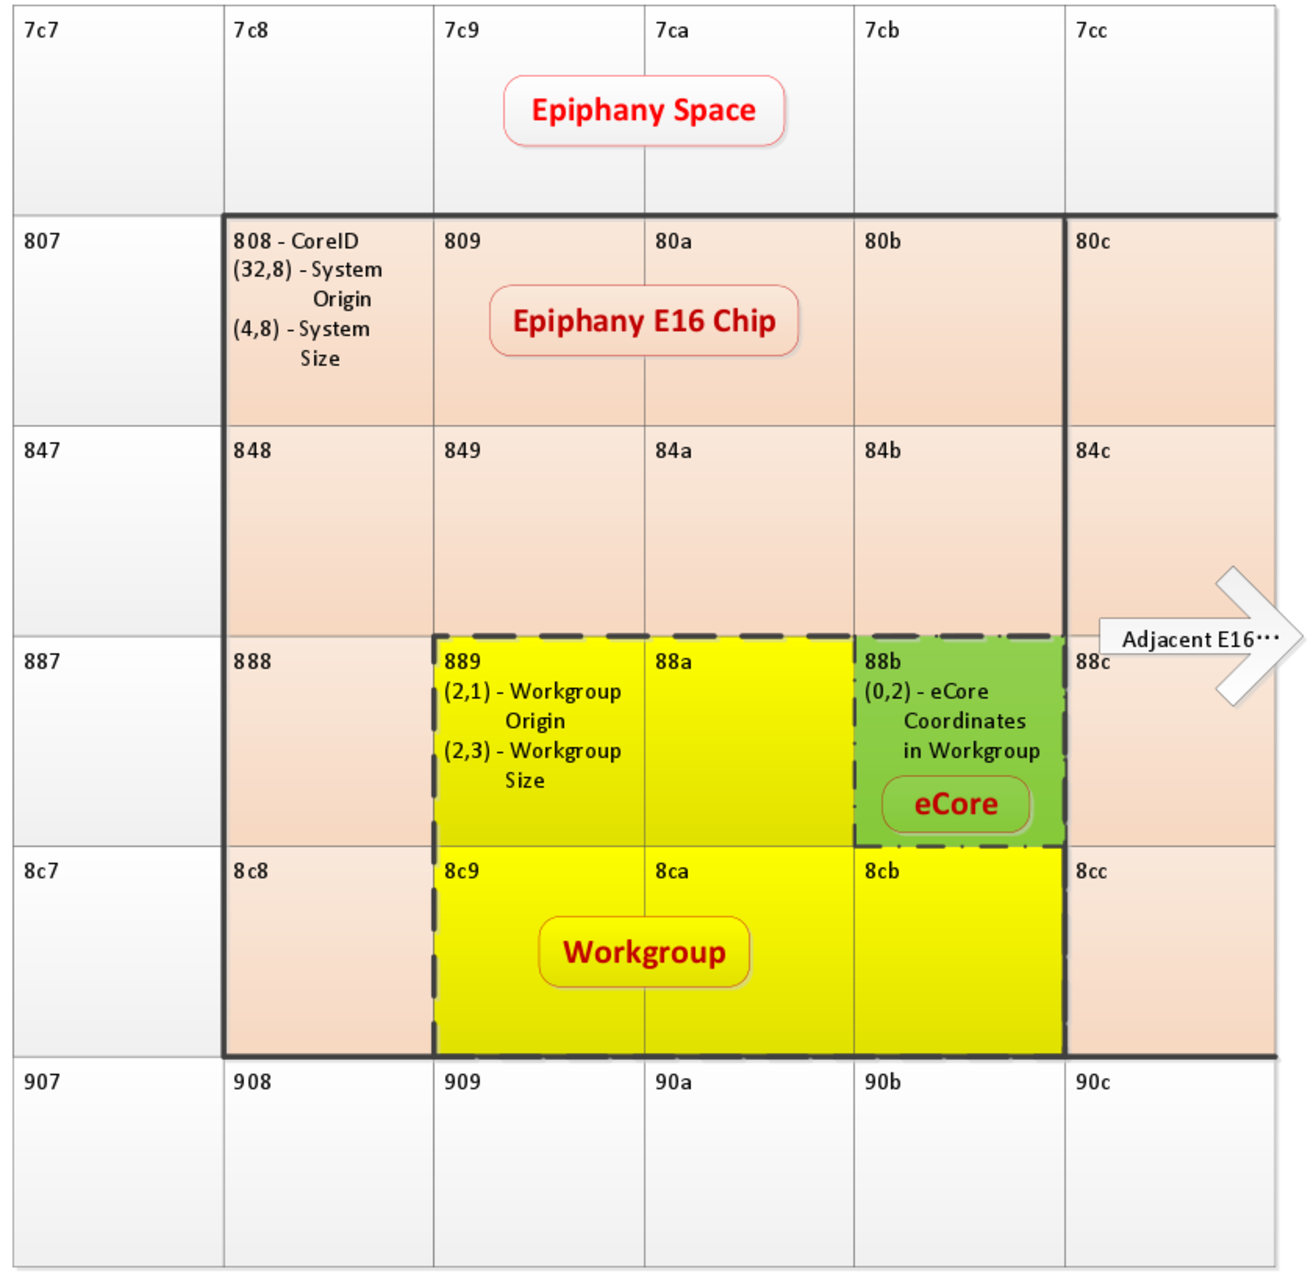
\includegraphics[scale=0.5]{EpiphanySpace.pdf}
\caption{The Epiphany\tm Platform, Workgroup an eCore coordinates. Source: Adapteva Inc. Epiphany\tm SDK Reference}
\end{figure}
\end{centering}

\section{A2: Installing \texttt{epiphany-bsp}}

\subsection{Prerequisites}

We use the 2014-08 release of the Epiphany\tm SDK (eSDK), notes on installing this can be found here: \url{https://github.com/adapteva/epiphany-sdk/wiki/Notes-on-the-2014.08-release}.

First of all, on Ubuntu Linux we have to install the following packages:
\begin{align*} 
    &\texttt{sudo apt-get install u-boot-tools gcc-4.8-arm-linux-gnueabihf g++-4.8-arm-linux-gnueabihf} \\
    &\texttt{\hspace{1 cm}> bison flex libgmp-dev libncurses-dev libmpc-dev libmpfr-dev texinfo xzip lzip}
\end{align*}
Next, after cloning the \verb+epiphany-sdk+ repoistory we checkout the \texttt{2014.08.rc} branch.

When downloading the toolchain, we \verb+--clone+ to make sure we obtain the latest sources (allegedly else it will download outdated ones). Else the toolchain will then build for the build machine, but it might complain along the lines of \texttt{archive has no index}. We run \texttt{arm-linux-gnueabihf-ranlib} for all these archives to try and fix this, but to no avail...


\subsection{Obtaining the source}

\subsection{Example usage}

\section{References}

\begin{enumerate}
    \item \url{http://www.adapteva.com/white-papers/building-the-worlds-first-parallella-beowulf-cluster/}
    \item \url{http://www.adapteva.com/}
    \item \url{http://www.parallella.org}
    \item \url{MulticoreBSP}
    \item \url{BSPlib}
\end{enumerate}

\section{TODO}

Make epiphany-examples shared, symbolic link home folders abe jw
Memory Management


\end{document}
